\documentclass[20pt,landscape,dvips]{foils} 
% add 'draft' option above to exclude image when compiling
\usepackage[french]{babel}
\usepackage[utf8]{inputenc}  
\usepackage[french=guillemets*]{csquotes} 
\MakeOuterQuote{"}
\frenchspacing
\DecimalMathComma

\usepackage{latexsym}
\usepackage{amsmath,amssymb,amsfonts}
\usepackage{MnSymbol}
\usepackage{url}
\usepackage{graphicx}
%\usepackage[dvipsnames]{xcolor}
\usepackage{hyperref}
\usepackage{alltt}
\usepackage{pifont,manfnt}
\usepackage[dvipsnames,table]{xcolor}
\usepackage{subfig}
%\usepackage{enumerate}
%\usepackage{colortbl}
\usepackage{multirow,hhline}
\usepackage{cclicenses}
\setlength\parindent{0pt}
\hypersetup{colorlinks=true,citecolor=black,urlcolor=black,linkcolor=black}
\usepackage[style=verbose]{biblatex}
\bibliography{refs}

\newcommand{\highlight}[1]{\textcolor{Plum}{\bfseries #1}}
\newcommand{\remark}[1]{%
%\centerline{
\begin{center}
\framebox[.9\textwidth][t]{
\ding{46} 
\parbox[t]{.8\textwidth}{\small #1}}
\end{center}}

\DeclareMathOperator*{\inlaw}{\sim}
\newcommand{\iid}{\inlaw_{\text{i.i.d.}}}
%\newcommand{\iid}{\mathop{\mathrm{diag}}}
\newcommand{\pobs}{p_{\text{obs}}}

\reversemarginpar
\def\mark{\marginpar{\dbend}}

%\newcommand{\bm}[1]{\mbox{\boldmath{$#1$}}}
\renewcommand{\abstractname}{Summary}
\newcommand\bs{\char '134}   %  a backslash character for the \tt font
%\renewcommand\refname{Additional Readings}

% customize header/footer
\rightheader{}
% Note about the copyleft symbol:
% I use a custom reversed and circled "c" char because \textcopyleft in
% the textcomp package does not support sans serif font.
% Also, "c" is shifted horizontally by 1ex to align with the circle.
%\Restriction{\mbox{\raisebox{1.5ex}{\rotatebox{180}{\textcircled{c\kern.1ex}}} 2009}, \url{www.aliquote.org}}
% now I use the CC licence...
% \Restriction{\cc 2016 \VCRevision}
\Restriction{\cc 2016 Module 11 EESPE}

\title{Méthodes psychométriques en qualité de vie}
\author{Christophe Lalanne\\EA 7334 REMES\\ Unité de Méthodologie des critères d’évaluation\\Université Paris-Diderot, Sorbonne Paris-Cité\\}
\date{
\includegraphics[height=18ex]{logo.eps}}

%%% This file has been generated by the vc bundle for TeX.
%%% Do not edit this file!
%%%
%%% Define Git specific macros.
\gdef\GITHash{f4328f7906d309e9224e3e5c2f7f36477f44e69f}%
\gdef\GITAbrHash{f4328f7}%
\gdef\GITParentHashes{136657e4877819e72dc9ebb2f209631a2a8d1057}%
\gdef\GITAbrParentHashes{136657e}%
\gdef\GITAuthorName{Christophe Lalanne}%
\gdef\GITAuthorEmail{ch.lalanne@gmail.com}%
\gdef\GITAuthorDate{2016-07-06 10:29:58 +0200}%
\gdef\GITCommitterName{Christophe Lalanne}%
\gdef\GITCommitterEmail{ch.lalanne@gmail.com}%
\gdef\GITCommitterDate{2016-07-06 10:29:58 +0200}%
%%% Define generic version control macros.
\gdef\VCRevision{\GITAbrHash}%
\gdef\VCAuthor{\GITAuthorName}%
\gdef\VCDateRAW{2016-07-06}%
\gdef\VCDateISO{2016-07-06}%
\gdef\VCDateTEX{2016/07/06}%
\gdef\VCTime{10:29:58 +0200}%
\gdef\VCModifiedText{\textcolor{red}{with local modifications!}}%
%%% Assume clean working copy.
\gdef\VCModified{0}%
\gdef\VCRevisionMod{\VCRevision}%


\begin{document}
\LogoOff
\maketitle
\rightfooter{\quad\textsf{\thepage}}



%---------------------------------------------------------------Slide-
\foilhead{Modèles de réponse à l'item}
\begin{itemize}
\item Cas des données binaires
\item Cas des items polytomiques
\item Invariance de mesure
\end{itemize}



%---------------------------------------------------------------Slide-
\foilhead{}

\begin{quote}
That the model is not true is certainly correct,
no models are--not even the Newtonian laws. (\dots) Models should
not be true, but it is important that they are applicable\autocite{rasch60}.  
\end{quote}

%---------------------------------------------------------------Slide-
\foilhead{Données d'illustration}

Échelle d'anxiété issue de la banque d'items calibrés développée dans le cadre
du projet PROMIS (\url{http://www.nihpromis.org}) : 29 items de type Likert (1 =
\enquote{Never}, 2 = \enquote{Rarely}, 3 = \enquote{Sometimes}, 4 =
\enquote{Often}, and 5 = \enquote{Always}) ; $N=706$ individus sélectionnés
aléatoirement en population générale\autocite{Pilkonis2011,Choi2011}.

La construction du questionnaire a été réalisée à partir de l'analyse de 140
questionnaires existants, et la réduction de l'échelle d'origine a été réalisée
à l'aide de techniques de type CFA et IRT.

%---------------------------------------------------------------Slide-
\foilhead{Méthodologie PROMIS}

{\centering 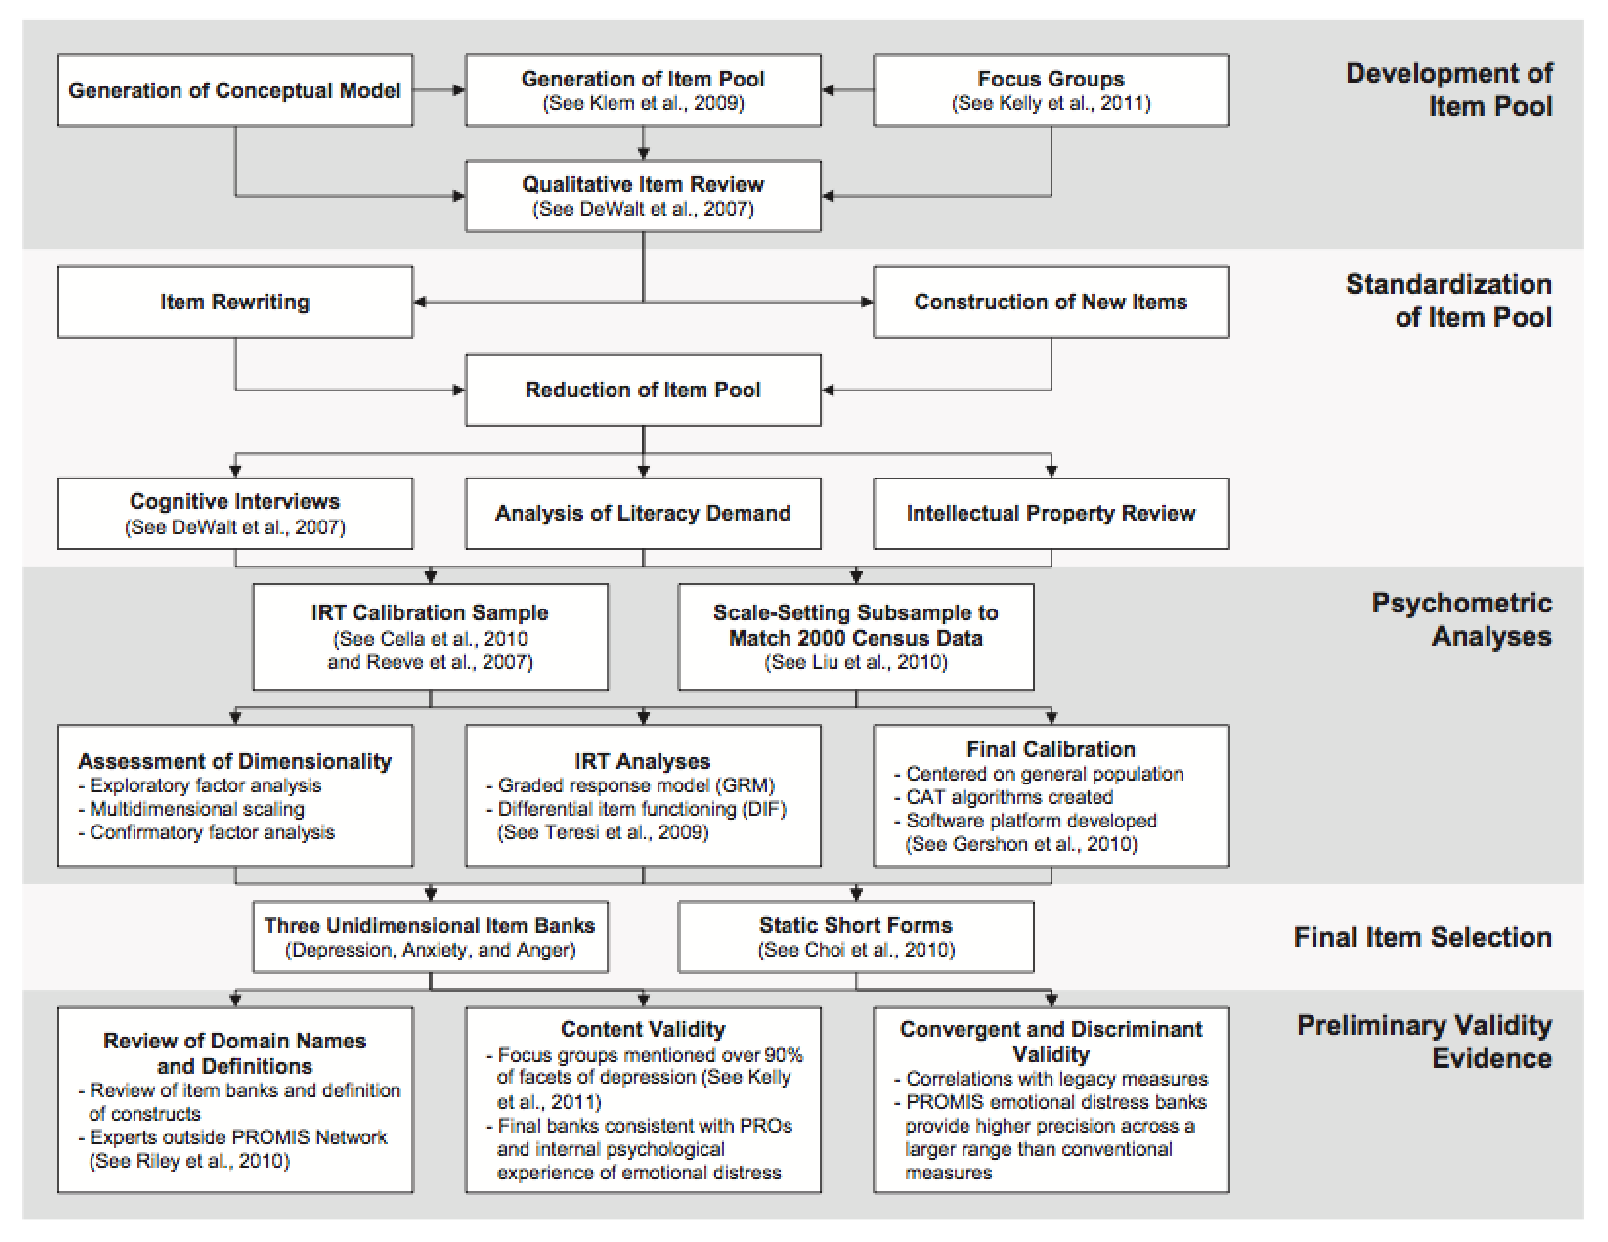
\includegraphics[width=.65\textwidth]{figs/promis.eps}\par}

%---------------------------------------------------------------Slide-
\foilhead{Contenu de l'échelle}

\begin{minipage}{0.45\textwidth}\scriptsize
\begin{enumerate}
\item I felt fearful
\item \highlight{I felt frightened}
\item It scared me when I felt nervous
\item \highlight{I felt anxious}
\item I felt like I needed help for my anxiety
\item I was concerned about my mental health
\item I felt upset
\item I had a racing or pounding heart
\item I was anxious if my normal routine was disturbed
\item \highlight{I had sudden feelings of panic}
\item I was easily startled
\item I had trouble paying attention
\item I avoided public places or activities
\item I felt fidgety
\item I felt something awful would happen
\newcounter{enumTemp}
\setcounter{enumTemp}{\theenumi}
\end{enumerate}
\end{minipage}\hfill
\begin{minipage}{0.45\textwidth}\scriptsize
\begin{enumerate}
\setcounter{enumi}{\theenumTemp}
\item \highlight{I felt worried}
\item \highlight{I felt terrified}
\item I worried about other people's reactions to me
\item I found it hard to focus on anything other than my anxiety
\item My worries overwhelmed me
\item I had twitching or trembling muscles
\item I felt nervous
\item I felt indecisive
\item Many situations made me worry
\item \highlight{I had difficulty sleeping}
\item I had trouble relaxing
\item I felt uneasy
\item I felt tense
\item I had difficulty calming down
\end{enumerate}
\end{minipage}

% ---------------------------------------------------------------Slide-
\foilhead{Analyse descriptive des fréquences de réponse}
\hfill $\triangleright$ anxiety.r

Données socio-démographiques : 397 femmes, 369 hommes, 555 âgés de moins de 65
ans.

{\centering 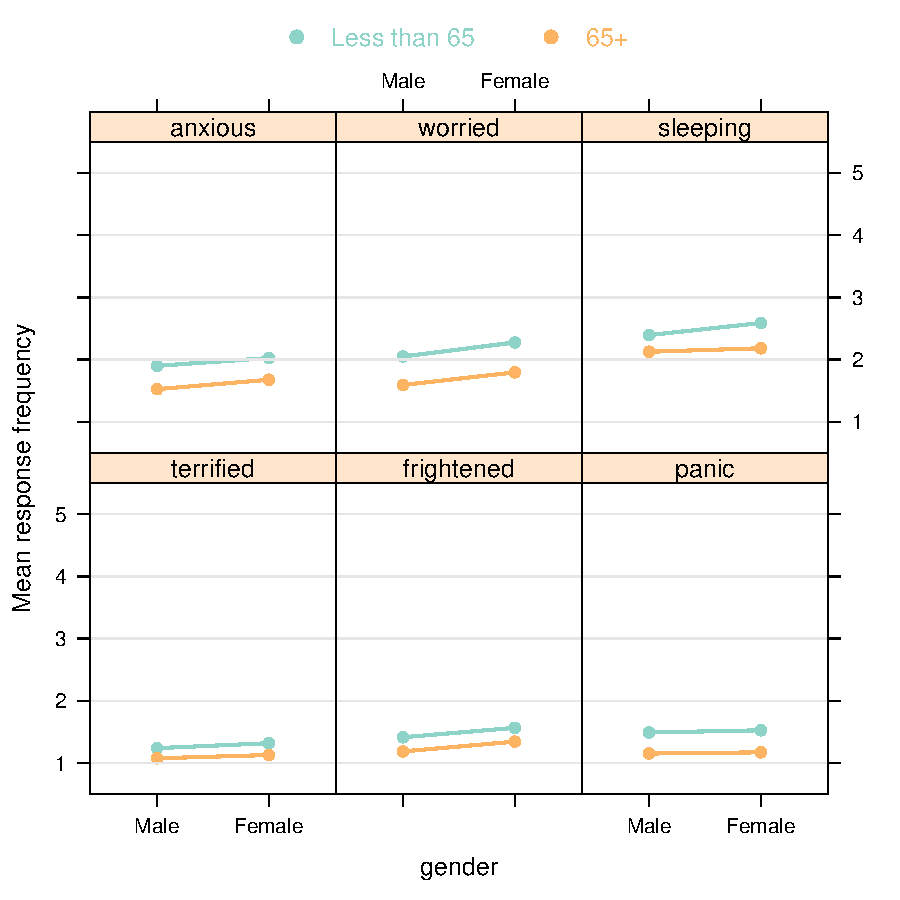
\includegraphics[width=.4\textwidth]{figs/anxiety_respfreq_by_gender.eps}\par}


% ---------------------------------------------------------------Slide-
\foilhead{Matrice de corrélations polychoriques}

{\centering 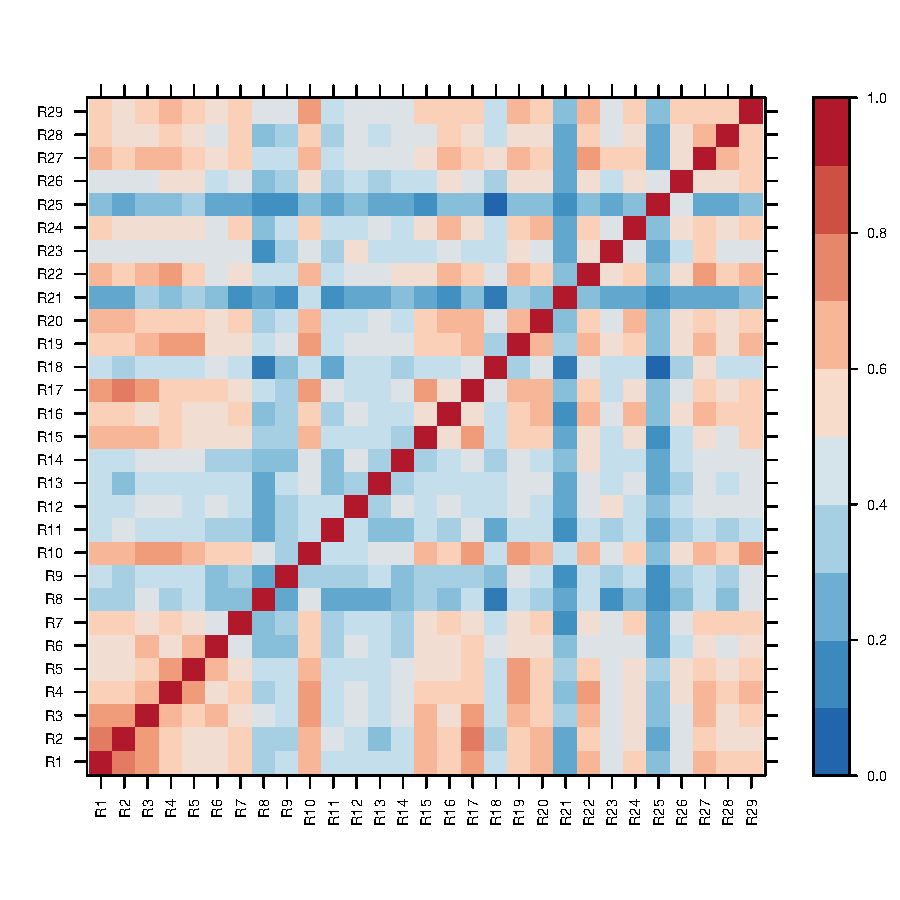
\includegraphics[width=.5\textwidth]{figs/anxiety_polychoric.eps}\par}


% ---------------------------------------------------------------Slide-
\foilhead{Distribution des valeurs propres de l'ACP}

{\centering 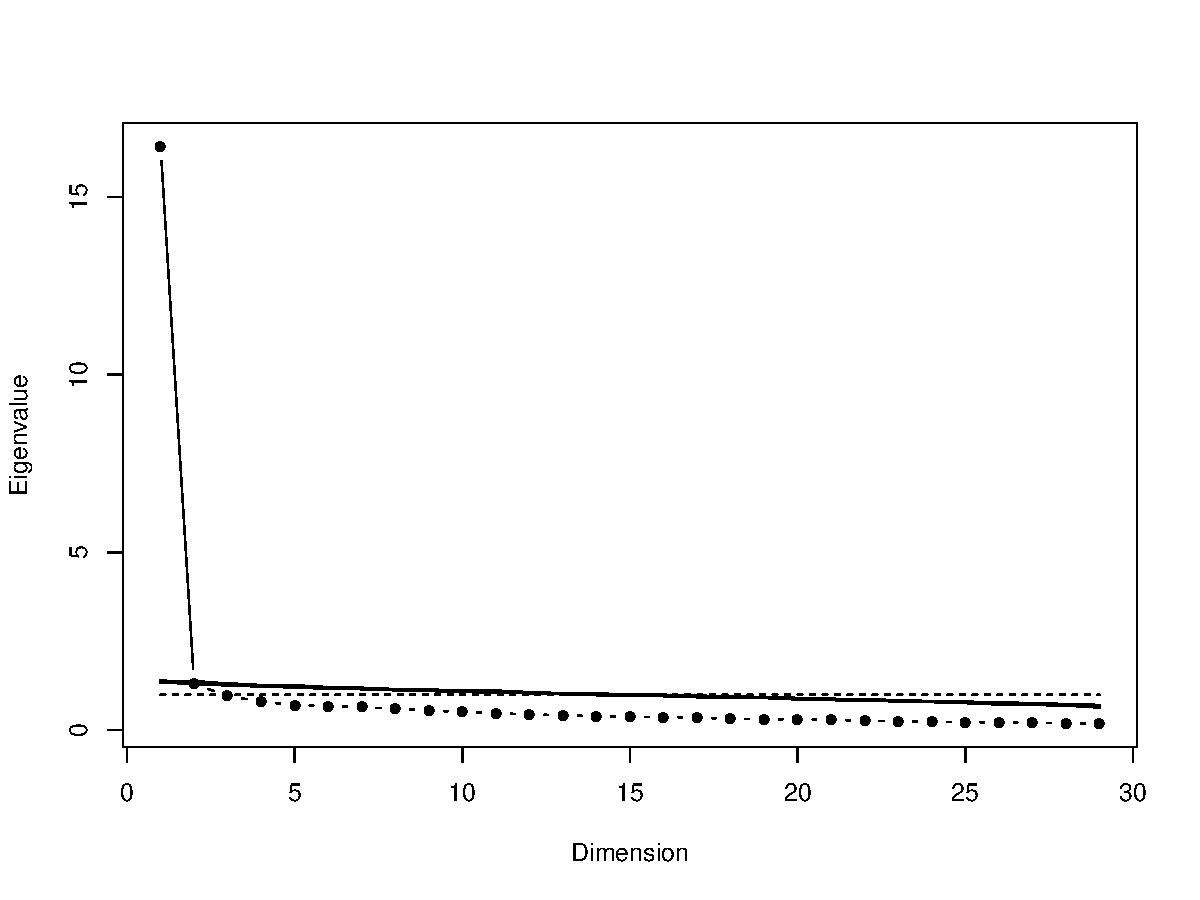
\includegraphics[width=.5\textwidth]{figs/anxiety_screeplot.eps}\par}

{\small Alpha de Cronbach = 0.971, IC 95~\% [0.967;0.975] (bootstrap)}


% ---------------------------------------------------------------Slide-
\foilhead{Scores totaux et scores factoriels}

{\centering 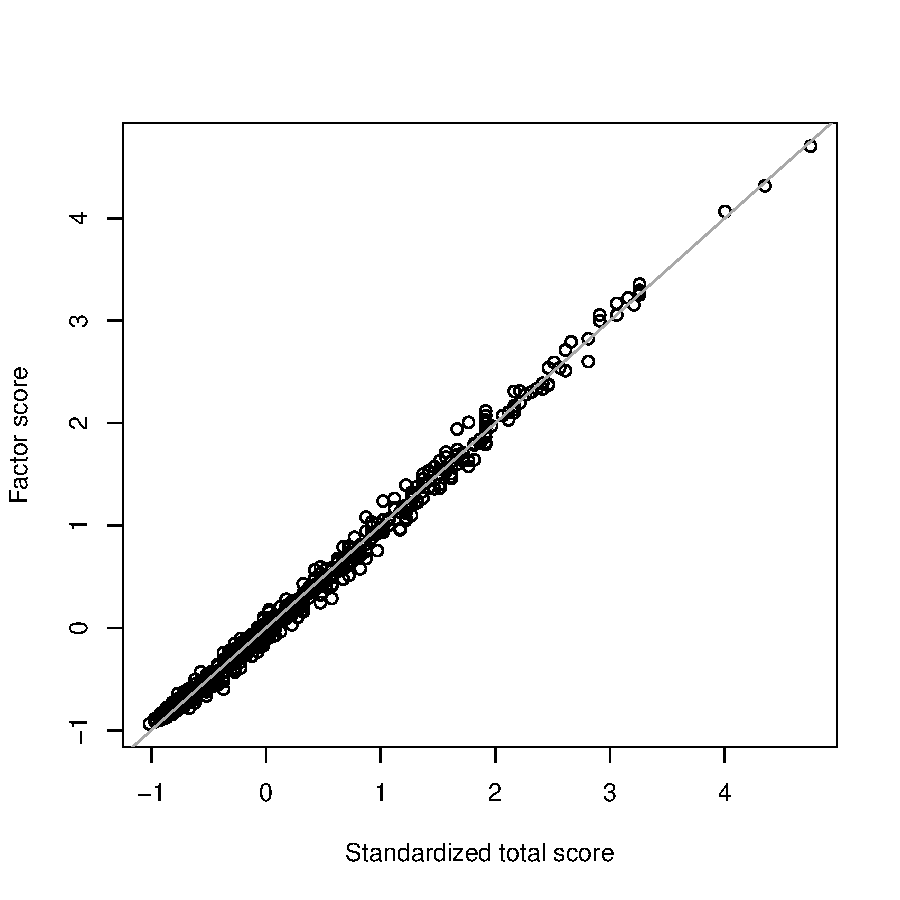
\includegraphics[width=.5\textwidth]{figs/anxiety_fa_scores.eps}\par}

% ---------------------------------------------------------------Slide-
\foilhead{Analyse sur données binaires (1/2 = 0, 3/5 = 1)}

On va appliquer un \enquote{modèle de Rasch}\autocite{RabeHesketh2008} qui
permet de modéliser conjointement la \enquote{difficulté} des items et
l'\enquote{habileté} des participants. Dans ce contexte, la difficulté
s'apparente à la sévérité du trouble anxieux, et l'habileté au niveau d'anxiété.
On fait explicitement l'hypothèse que l'ensemble des items ont un pouvoir
discriminant équivalent (absence d'interaction entre les deux paramètres).

La probabilité de réussite $P(X_j=1\mid \theta)$ à un item $j$ pour un
individu ayant une valeur $\theta$ d'habileté s'écrit simplement :
\[
P(X_j=1\mid \theta) = \frac{e^{\theta-\delta_j}}{1+e^{\theta-\delta_j}}.
\]

% ---------------------------------------------------------------Slide-
\foilhead{Distribution des fréquences de réponse}

{\centering \includegraphics[width=.5\textwidth]{figs/anxiety_respfreq.eps}\par}

% ---------------------------------------------------------------Slide-
\foilhead{Corrélation des réponses avec le score total}

{\centering \includegraphics[width=.8\textwidth]{figs/anxiety_biserial.eps}\par}

% ---------------------------------------------------------------Slide-
\foilhead{Valeurs estimés de difficulté des items}

{\centering 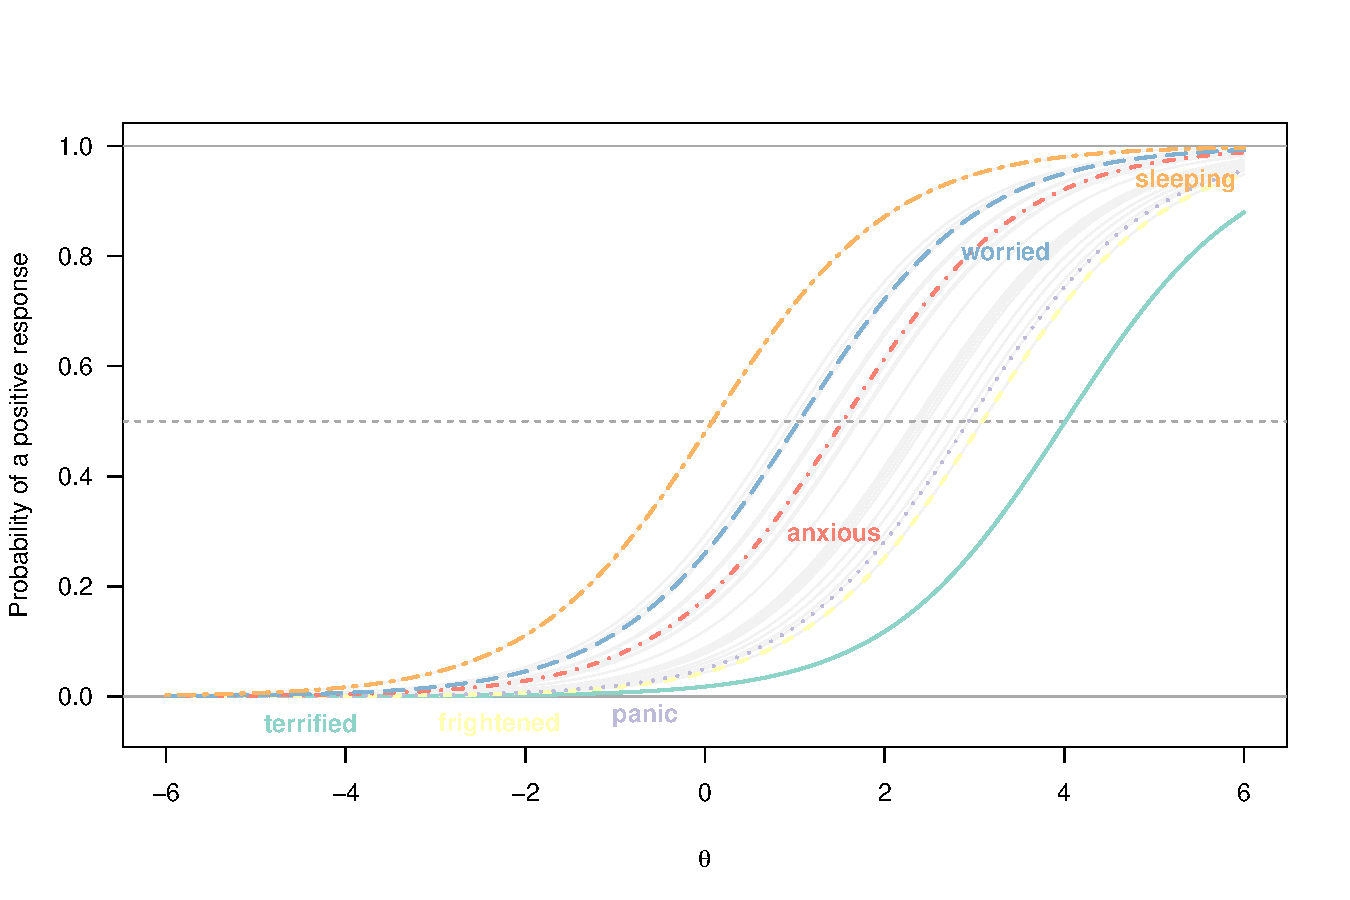
\includegraphics[width=.7\textwidth]{figs/anxiety_onepl.eps}\par}

% ---------------------------------------------------------------Slide-
\foilhead{Score total et score IRT}

Si les conditions d'application du modèle sont vérifiées, le score total est un
 proxy pour le score factoriel ($\theta$).

{\centering 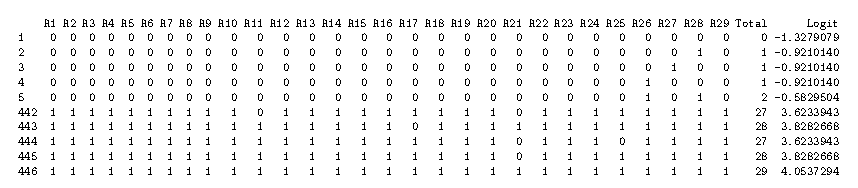
\includegraphics[width=\textwidth]{figs/anxiety_resp_patt.eps}\par}

Les 446 \highlight{patterns de réponse} permettent de calculer 30 scores distincts.

% ---------------------------------------------------------------Slide-
\foilhead{Relation entre score factoriel et score total}

{\centering \includegraphics[width=.5\textwidth]{figs/anxiety_rasch_scale.eps}\par}


% ---------------------------------------------------------------Slide-
\foilhead{Distribution jointe des items et des participants}

{\centering 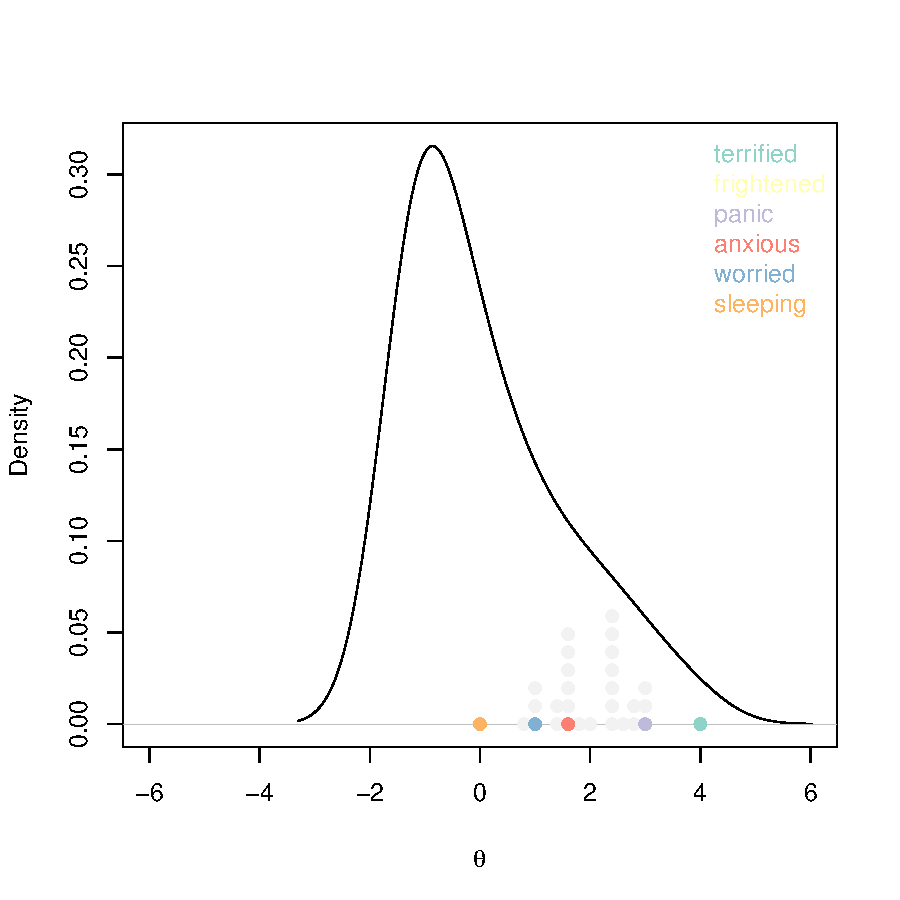
\includegraphics[width=.5\textwidth]{figs/anxiety_rasch_itmap.eps}\par}


% ---------------------------------------------------------------Slide-
\foilhead{Modèle à deux paramètres (difficulté et discrimination)}

{\centering 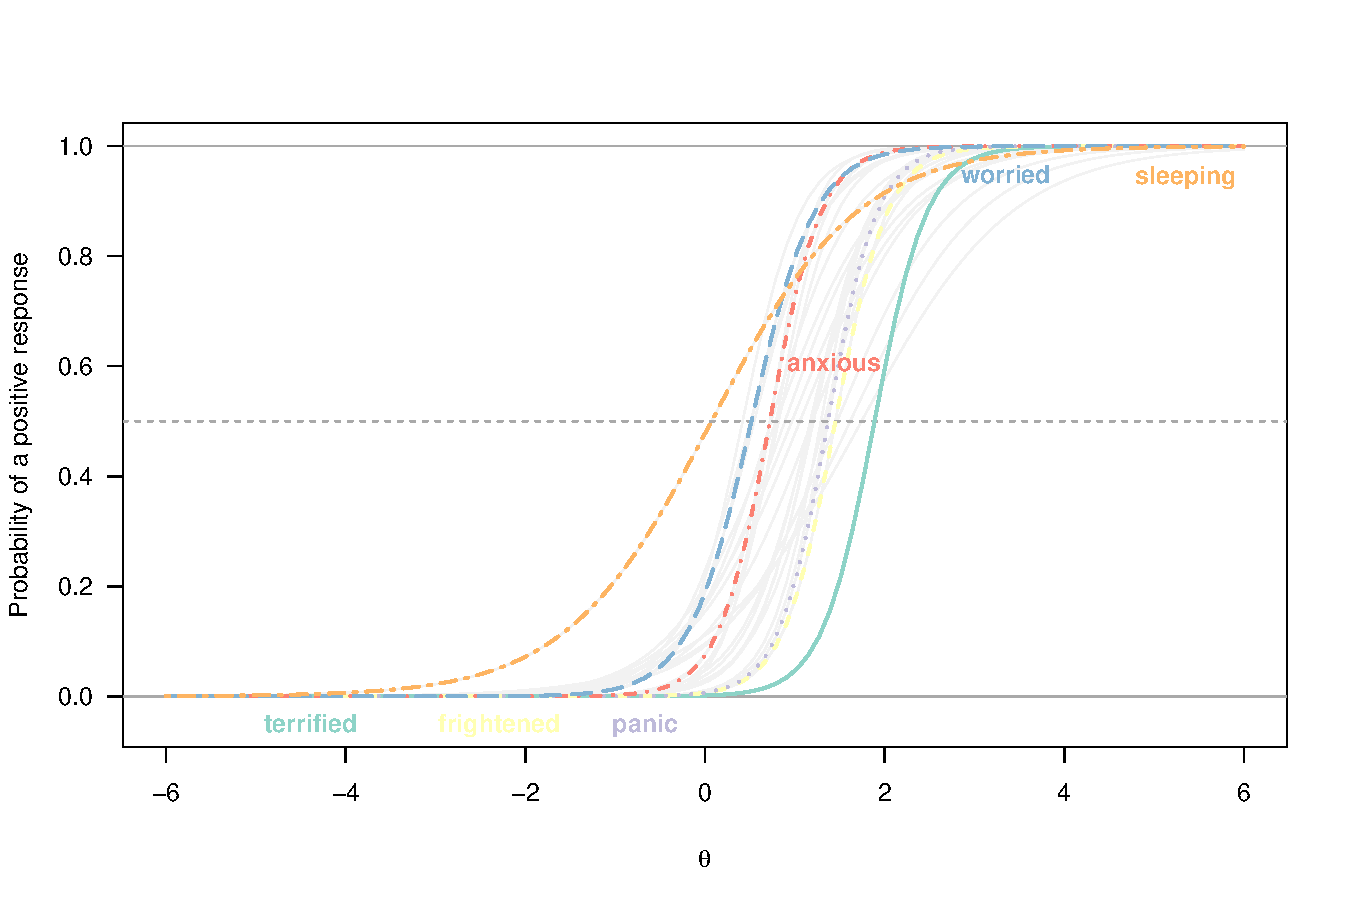
\includegraphics[width=.5\textwidth]{figs/anxiety_twopl.eps}\par}


% ---------------------------------------------------------------Slide-
\foilhead{Comparaison des paramètres de difficulté}

{\centering 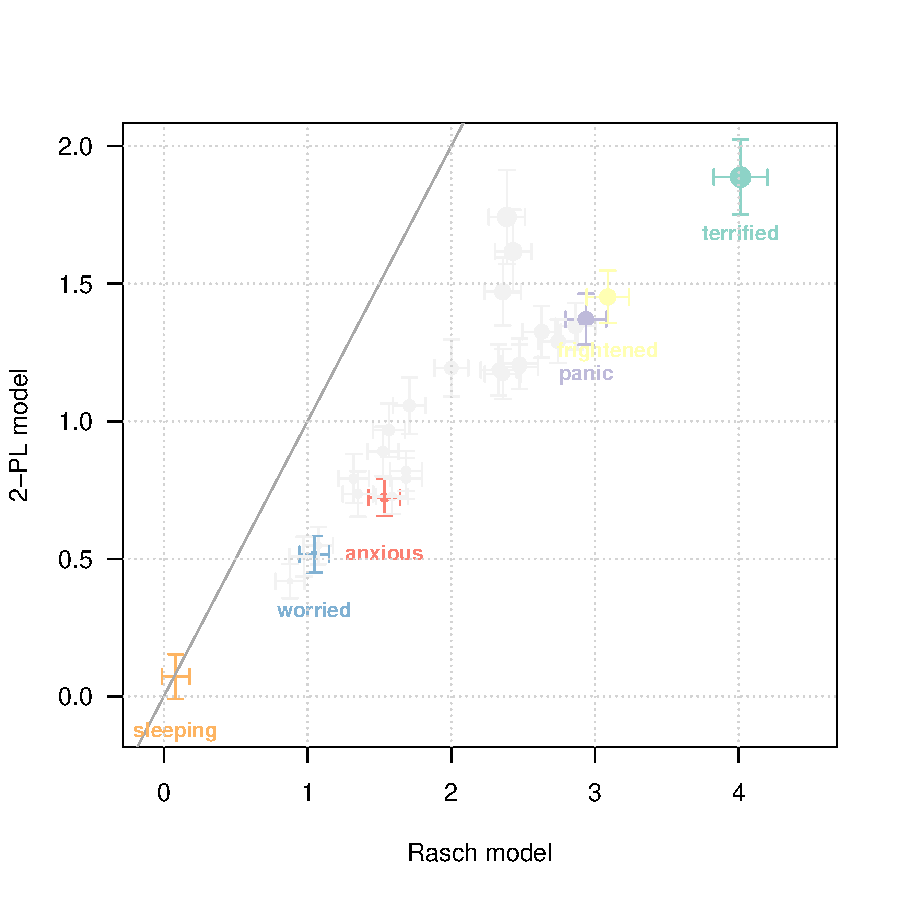
\includegraphics[width=.5\textwidth]{figs/anxiety_itemsdiff.eps}\par}


% ---------------------------------------------------------------Slide-
\foilhead{Extension : cas des items polytomiques}

Plusieurs modèles IRT ont été proposés pour analyser spécifiquement les items à
plus de deux modalités de réponse (ordonnées ou non), certains se situant dans
la tradition du modèle de Rasch, d'autres ayant des hypothèses plus souples
\autocite{Hays2000,rao06}. 

Pour illustration, voici les résultats de l'analyse à l'aide du modèle de
réponse graduée (GRM) \autocite{Samejima1969}.


% ---------------------------------------------------------------Slide-
\foilhead{}

{\centering \includegraphics[width=.8\textwidth]{figs/anxiety_grmcons_it1.eps}\par}

% ---------------------------------------------------------------Slide-
\foilhead{}

{\centering 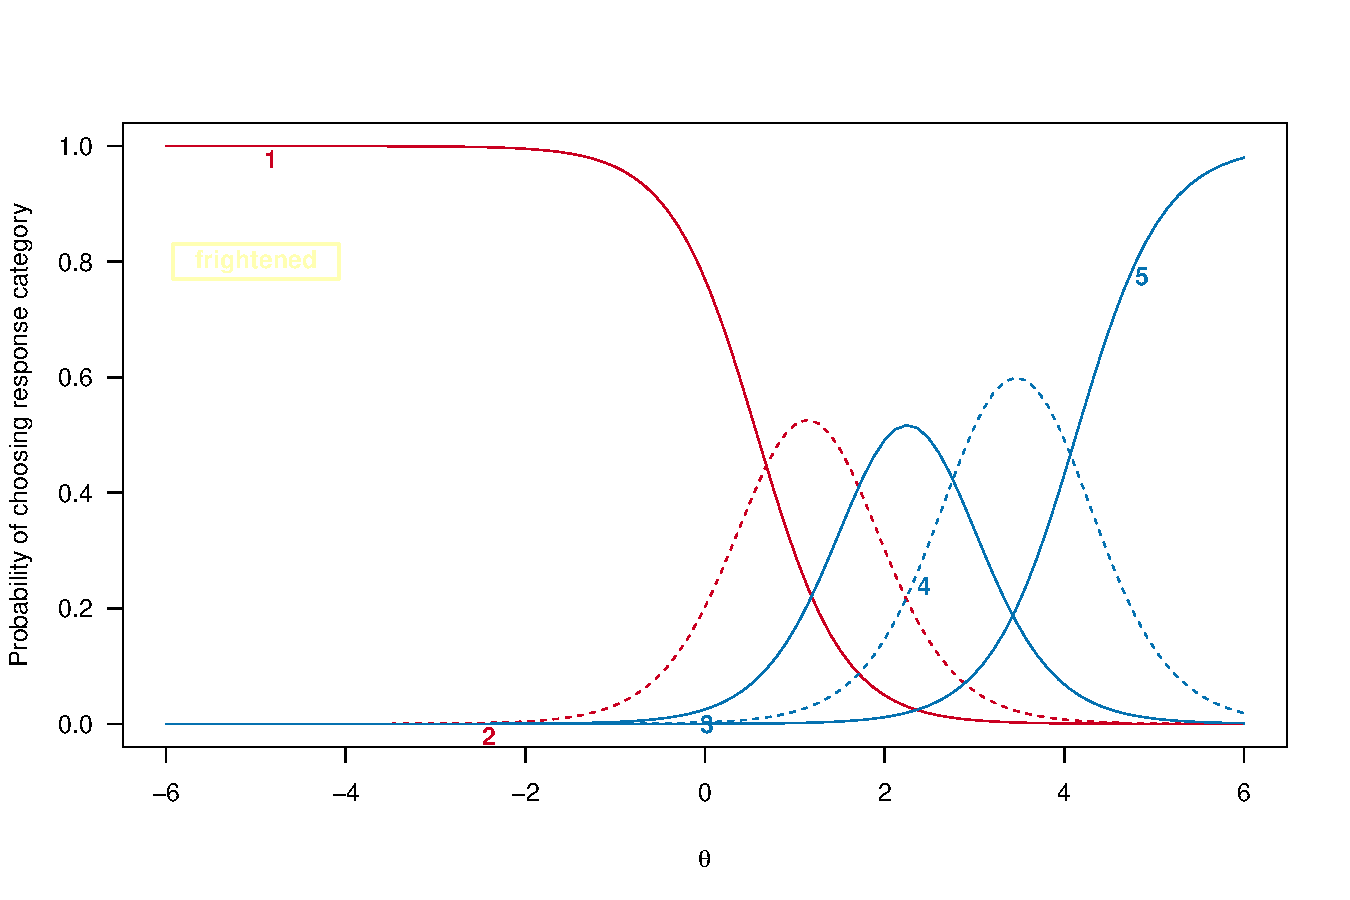
\includegraphics[width=.8\textwidth]{figs/anxiety_grmcons_it2.eps}\par}

% ---------------------------------------------------------------Slide-
\foilhead{}

{\centering 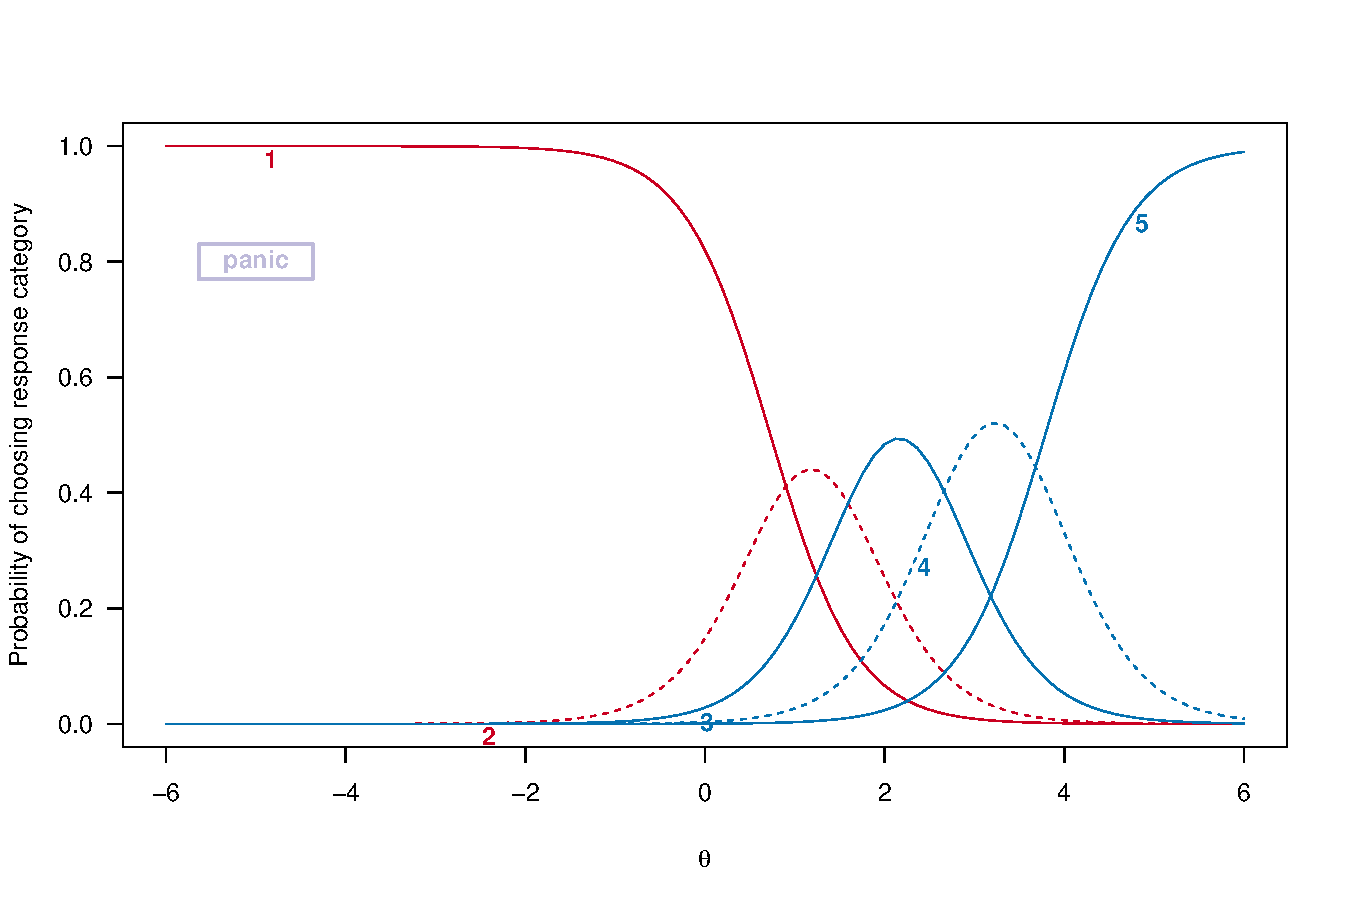
\includegraphics[width=.8\textwidth]{figs/anxiety_grmcons_it3.eps}\par}

% ---------------------------------------------------------------Slide-
\foilhead{}

{\centering 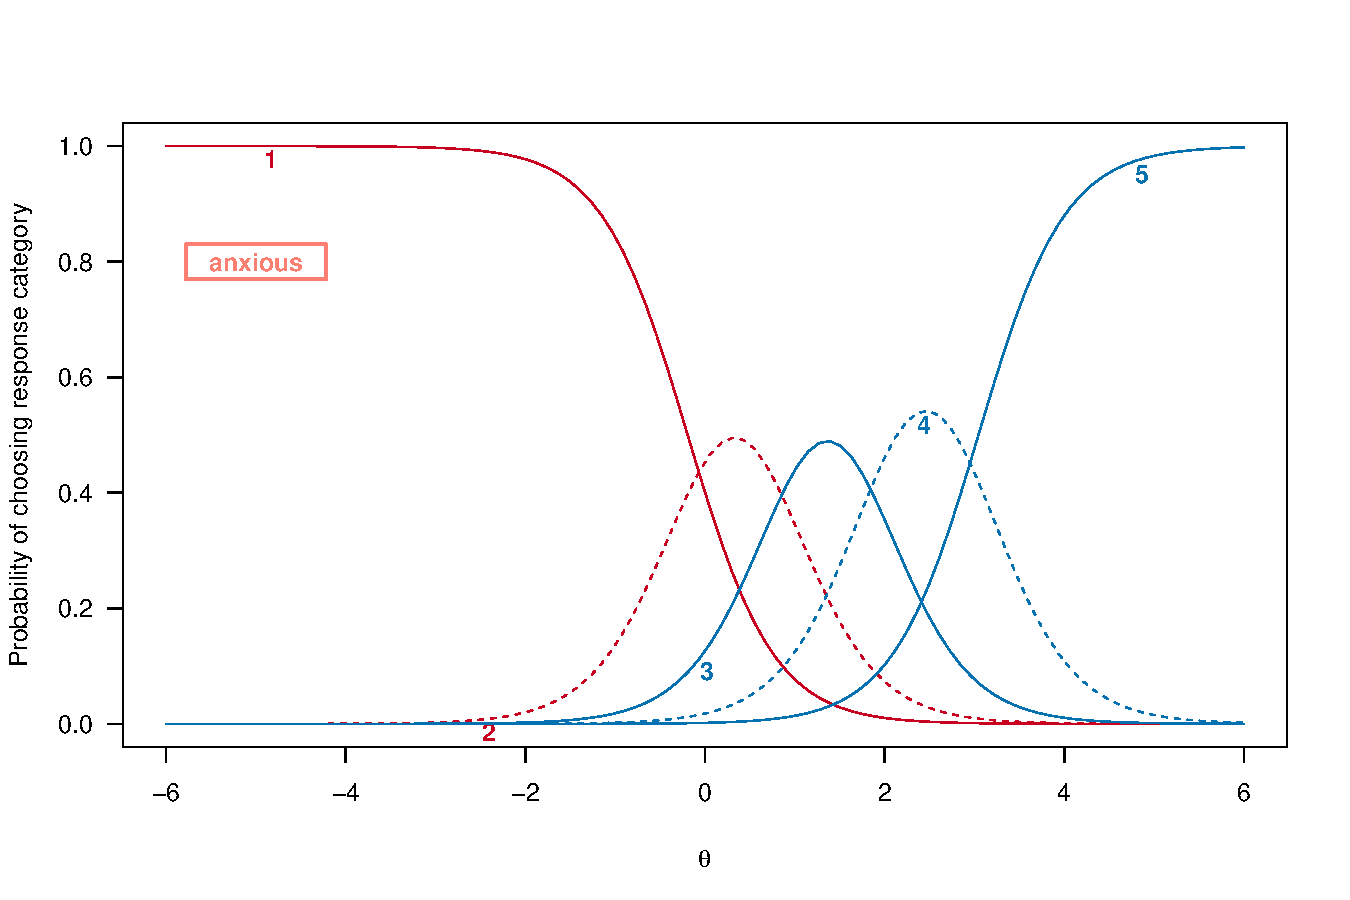
\includegraphics[width=.8\textwidth]{figs/anxiety_grmcons_it4.eps}\par}

% ---------------------------------------------------------------Slide-
\foilhead{}

{\centering 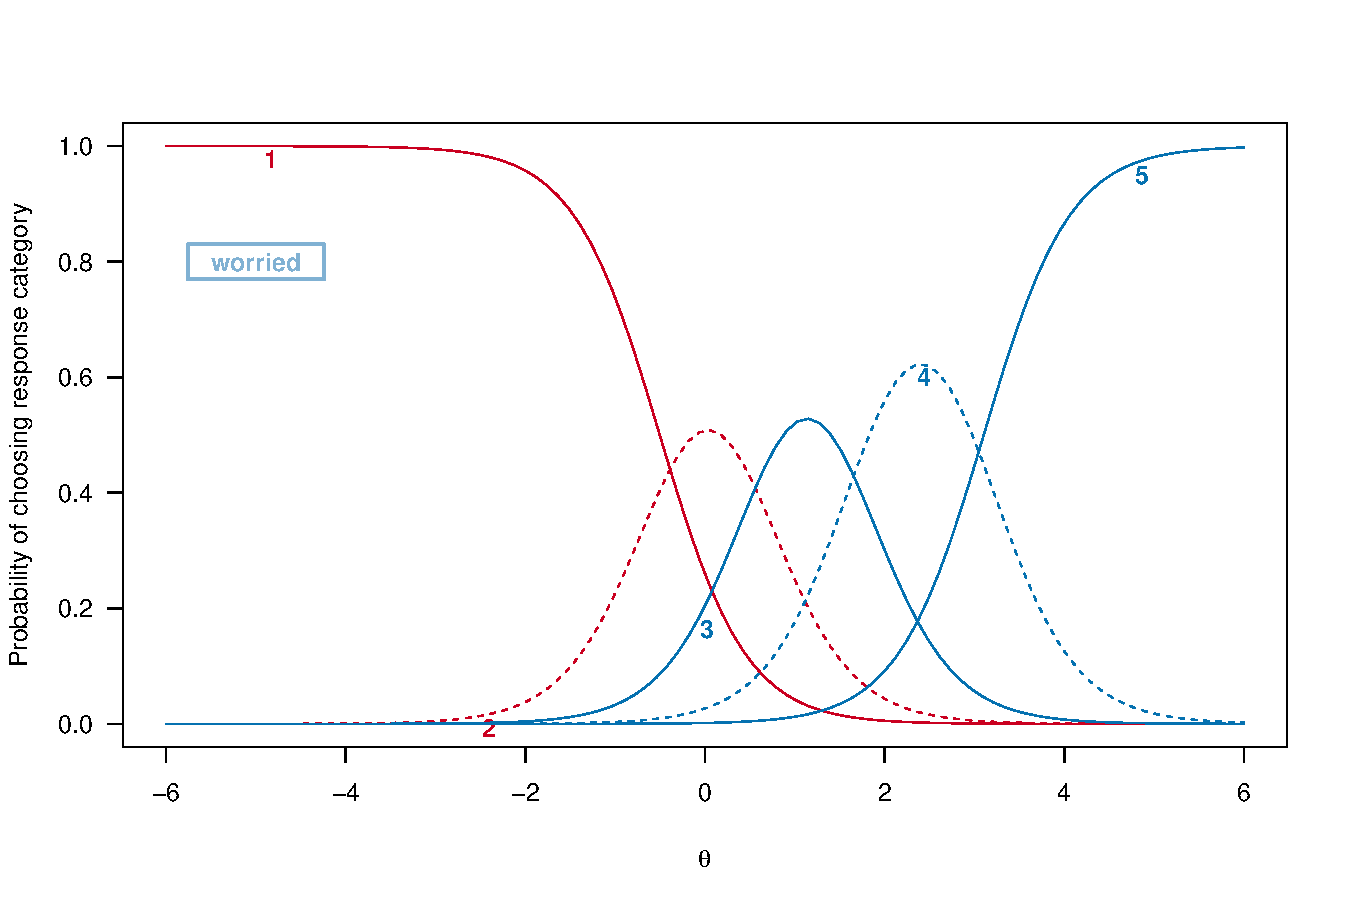
\includegraphics[width=.8\textwidth]{figs/anxiety_grmcons_it5.eps}\par}

% ---------------------------------------------------------------Slide-
\foilhead{}

{\centering \includegraphics[width=.8\textwidth]{figs/anxiety_grmcons_it6.eps}\par}


% ---------------------------------------------------------------Slide-
\foilhead{}

Fichier de données et scripts R disponibles à l'adresse suivante :\newline
{\centering \url{https://bitbucket.org/chlalanne/eespe11}\par}
\vfill

\raggedleft \scriptsize -- Typeset with \FoilTeX\ (version 2), Revision \VCRevision

\end{document}
